\chapter{Generative Adversarial Networks}
Many generative models are based on the idea of using a differentiable generator
network. The model transforms samples of latent variables $z$ to samples $x$ or
to distributions over samples $x$ using a differentiable function $g(z; \theta^{(g)})$,
which is typically represented by a neural network. This model class includes:
\begin{itemize}
    \item \textbf{Variational auto-encoders}: which pair the generator net with
          an inference net;
    \item \textbf{Generative Adversarial Networks} (GAN): which pair the generator
          network with a discriminator network;
    \item Techniques that train generator networks in isolation.
\end{itemize}

Generator networks are essentially just parametrized computational procedures for
generating samples, where the architecture provides the family of possible
distributions to sample from and the parameters select a distribution from within
that family.

The goal of this model is to generate something starting from random noise. In
order to do this, we want to create a model that is capable \textbf{to learn to
    sample} the distribution of the training set. Usually, this models are
unsupervised because they do not use a labels because we haven't any information
on that.

Its possible to create model that are able to generate a new sample based on some
condition, for examples generating a new instance starting from a given label.
Moreover, this models can be use for \textit{image to image translation}. In this
case we solve task like given a black\&white image and we want to generate the
colored image. This feature makes these models very useful for performing computer
vision tasks such as: increasing data, improving image, etc$\dots$

In order to build a generative model we need two main components:
\begin{itemize}
    \item The first is to define an architecture that allows a new sample to be
          generated.
    \item The second is to define the correct loss function.
\end{itemize}
So we want to learn to sample, so $x \sim p_{data}$ should be $x_{gen}\sim p_{model}$,
such manner that $p_{data} \equiv p_{model}$.
\section{Generator architecture}
During this course, we have already explored a type of neural network capable of
generating data: the \textit{autoencoder}. Specifically, by isolating the decoder
component and sampling from the latent space, we can generate novel examples.

Up to this point we have only seen architectures that allow to reduce the size
of the images (CNN). We want to see how we can use these architectures to up-sample
from  a noise distribution. We start from a convolution like the one shown in
figure \ref{fig:reg-conv}

\begin{figure}[!ht]
    \centering
    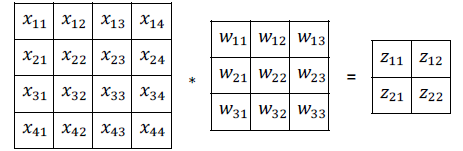
\includegraphics[width=0.5\linewidth]{img/GAN/RegularConv.png}
    \caption{Regular convolution stride 1, pad 0}
    \label{fig:reg-conv}
\end{figure}

We can rewrite this operation in a matrix form figure \ref{fig:conmat}.

\begin{figure}[!ht]
    \centering
    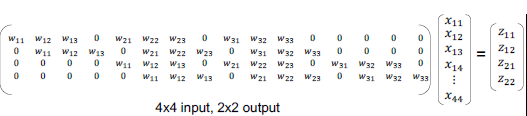
\includegraphics[width=0.5\linewidth]{img/GAN/matrix-vector.png}
    \caption{Matrix form}
    \label{fig:conmat}
\end{figure}

From here we realize that we can increase the size if we multiply our result by
the transposition of the filter figure \ref{fig:traConv}. It is necessary to note
that this operation \textbf{does not correspond to the inverse} of the original
convolution.

\begin{figure}[!ht]
    \centering
    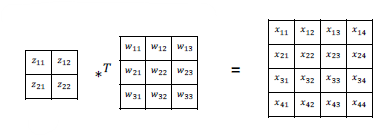
\includegraphics[width=0.5\linewidth]{img/GAN/transposeConv.png}
    \caption{Caption}
    \label{fig:traConv}
\end{figure}

The figure \ref{fig:TConvRes} shows the result of this operation at the graphic level.

\begin{figure}[!ht]
    \centering
    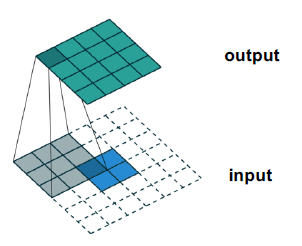
\includegraphics[width=0.5\linewidth]{img/GAN/results.png}
    \caption{Caption}
    \label{fig:TConvRes}
\end{figure}

Generative adversarial networks are based on a game theoretic scenario in which
the generator network must compete against an adversary. The generator network
directly produces samples $x = g(z; \theta^{(g)})$. Its adversary, the
\textbf{discriminator network}, attempts to distinguish between samples drawn
from the training data and samples drawn from the generator. The discriminator
emits a probability value given by $d(x; \theta^{(d)})$, indicating the
probability that $x$ is a real training example rather than a fake sample drawn
from the model.
\section{Define the loss function}
The simplest way to formulate learning in generative adversarial networks is as
a zero-sum game, in which a function $v(\theta^{(g)}, \theta^{(d)})$ determines
the payoff of the discriminator. The generator receives $- v(\theta^{(g)}, \theta^{(d)})$
as its own payoff. During learning, each player attempts to maximize its own
payoff, so that at convergence:
\begin{equation}
    g^\ast = \arg \min_{g} \max_{d} v(g, d)
\end{equation}
With this approach we are training the generator and the discriminator jointly
in a \textbf{minimax game}, where both need to get better and better to improve
the generation quality.

The default choice for $v$ is:
\begin{equation}
    V(\theta^{(g)}, \theta^{(d)}) = \mathbb{E}_{x \sim p_{data}} \log d(x) + \mathbb{E}_{z \sim p_{model}} \log(1 - d(g(z)))
\end{equation}
This drives the discriminator to attempt to learn to correctly classify samples
as real or fake, in other words the discriminator wants to maximize:
\begin{equation*}
    d^\ast = \arg \max_d V(g,d)
\end{equation*}
Simultaneously, the generator attempts to fool the classifier into believing its
samples are real:
\begin{equation*}
    G^\ast = \arg \min_G V(G,D)
\end{equation*}

In general, simultaneous gradient descent on two players' costs is not guaranteed
to reach an equilibrium. Note that the equilibria for a minimax game are not
local minima of $v$. Instead, they are points that are simultaneously minima for
both players' costs. This means that they are \textit{saddle points} of $v$ that
are local minima with respect to the first player's parameters and local maxima
with respect to the second player's parameters.

The training process therefore consists of alternating between:
\begin{itemize}
    \item Gradient ascent on discriminator:
          \begin{equation}
              D^\ast = \arg \max_D V(G,D)
          \end{equation}
    \item Gradient descent on generator (minimize log-probability of discriminator being right):
          \begin{equation}
              G^\ast = \arg \min_G V(G,D) = \arg \min_G \mathbb{E}_{z\sim p_{gen}} \log(1-D(G(z)))  =  \arg \max_G \mathbb{E}_{z\sim p_{gen}} \log(D(G(z)))
          \end{equation}
\end{itemize}

\begin{figure}[!ht]
    \centering
    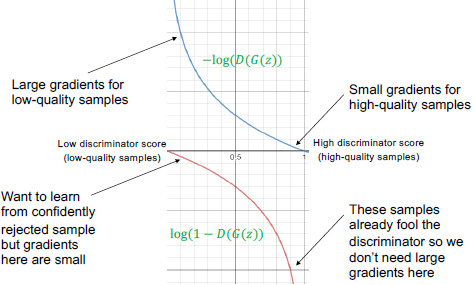
\includegraphics[width=0.5\linewidth]{img/GAN/loss.png}
    \caption{Loss function}
    \label{fig:lossfunc}
\end{figure}

In the original version the loss of the generator $G$ learns fewer from initial
image generated, but in this moment we want to learn more, the opposite thing
happen for higher value of the discriminator and this isn't useful. So we rewrite
the loss function using  $1 - \log(D(G(z)))$ in order to learn more at the
starting of the training.

The process for updating the generator increase $D(G(z))$ requires back-propagating
through the composed generator-discriminator network i.e., the discriminator
cannot be a black box. The generator is exposed to real data only via the output
of the discriminator and its gradients.

GANs have different problems:
\begin{itemize}
    \item \textbf{Unstability}: parameters can oscillate or diverge, generator
          loss does not correlate with sample quality and the behavior is sensitive to
          hyper-parameter selection
    \item \textbf{model collapse}: the generator ends up modeling only a small
          subset of the training data and not the entire distribution
\end{itemize}

Here some tips on GAN:
\begin{itemize}
    \item \textbf{conditional GAN}: It is possible to train conditional GANs that learn
          to sample from a distribution $p(x | y)$ rather than simply sampling from a
          marginal distribution $p(x)$.
    \item \textbf{Non-Saturating Generator Loss}: using the original generator loss
          when the discriminator can recognize each fake examples, this means that
          $D(G(X))$ is close to $0$ so $\log(1-D(G(X)))$ is close to 0 and the Generator
          can't learn. We can use Non-Saturating Generator Loss that solve this problem
          by maximizing $\log(D(G(X)))$. Another tip to solve this problem is to set
          threshold of real example lower, ex: $0.9$ instead of $1$ in discriminator.
    \item \textbf{class-label discriminator}: If we have a dataset of C classes
          we can use a discriminator that try to classify data between C+1 classes, where
          the C+1 class is the fake one. Empirically improves generation quality because
          the discriminator focus on features that are important for humans.
    \item \textbf{Virtual batch norm}: Batch normalization typically normalizes
          data within each mini-batch during training, but this can cause issues in GANs
          because can add instability and also artifacts. We can use Virtual batch norm
          which use a reference batch used for compute statistics and use them to normalized
          the actual mini-batch.
    \item \textbf{Mini-batch discrimination}: using a discriminator that use just
          an example cannot detect model collapse, we can solve by adding to any
          images some features derived from entire mini-batch.
\end{itemize}

\section{Evaluating Generative Models}
Generative modeling is different from normal model because changes in preprocessing,
even very small and subtle ones, are completely unacceptable. Any change to the
input data changes the distribution to be captured and fundamentally alters the task.

Because being able to generate realistic samples from the data distribution is
one of the goals of a generative model, practitioners often evaluate generative
models by visually inspecting the samples. Unfortunately, it is possible for a
very poor probabilistic model to produce very good samples. Imagine a generative
model trained on images of dogs and cats that simply learns to reproduce the
training images of dogs. Such a model has clearly overfit, because it does not
produces images that were not in the training set, but it has also underfit,
because it assigns no probability to the training images of cats. Yet a human
observer would judge each individual image of a dog to be high quality. In more
realistic settings, a generative model trained on data with tens of thousands of
modes may ignore a small number of modes, and a human observer would not easily
be able to inspect or remember  enough images to detect the missing variation.

Since the visual quality of samples is not a reliable guide, we often also evaluate
the log-likelihood that the model assigns to the test data, when this is
computationally feasible. Unfortunately, in some cases the likelihood seems not
to measure any attribute of the model that we really care about.

The fact that there are many different uses of generative models the choice of
metric must match the intended use of the model.


We pass from discriminator to update a generator because we don't know which loss
put in output to generator.